\chapter{初等几何：从测量、作图到证明}

前两章里，我们用字母和方程把许多具体问题压缩成了可以搬运的模型。那些问题大多发生在“数量”的世界里：价格、速度、时间。这一章我们要换一个世界——形状的世界。你将看到，人类最早的几何知识来自非常实际的需要：丈量土地、建造房屋、观察星空。但这门学科最惊人的地方在于，它最终挣脱了尺子和绳子的限制，变成了一门只凭推理就能保证结论的学问。这是数学史上第一次出现“证明”，也是整本书反复回响的主题第一次登场。

\section{影子里的金字塔}

大约两千六百年前，一位旅行者来到埃及。他站在巨大的金字塔前，问了一个让当地祭司发愣的问题：这座塔有多高？

直接测量是不可能的。塔身是石头砌成的斜面，没有梯子能爬到尖顶，把绳子从塔顶垂下来也做不到——那时没有任何工具能够到一百多米高的顶点。旅行者没有爬塔，他只要了一根木杆、一段绳子和一个晴天。

他把木杆竖直插在地上，等阳光照下来。木杆在地上投下一段影子，金字塔也在沙地上投下一大片阴影。他量了三个数：木杆的高度，木杆影子的长度，以及金字塔影子的长度（从塔底边缘量到阴影的尖端，再加上塔底边长的一半，因为塔的中心才是塔顶正下方的点）。然后他用一个简单的比例算出了金字塔的高度，据说误差很小。

这位旅行者就是古希腊的泰勒斯。传说中祭司们大为惊讶，但请你先别急着佩服他。这个故事里藏着一个真正的数学问题，它是本章的起点。

\section{为什么可以，为什么不可以}

泰勒斯的做法为什么是对的？他的直觉大概是：同一时刻，太阳光以相同的角度斜射下来，所以“木杆和它的影子”组成的小三角形，与“金字塔和它的影子”组成的大三角形，是同一个形状的放大版。形状相同，对应边的比例就相同，于是

\[
\frac{\text{金字塔高}}{\text{木杆高}}=\frac{\text{金字塔影长}}{\text{木杆影长}}.
\]

四个量里知道三个，第四个就能算出来。比如木杆高 $2$ 米，影长 $3$ 米，金字塔影长（折算到塔中心）$180$ 米，那么金字塔高就是 $2\times 180\div 3=120$ 米。

这个推理听起来很自然。但请停下来，像数学家那样多问一句：凭什么“形状相同”就能推出“对应边成比例”？这件事你量一百个三角形都会觉得对，可“量着对”和“一定对”之间隔着一条鸿沟。

先看一个容易上当的例子。画一个三角形，用量角器量它的三个内角，加起来是多少？多半不是正好 $180^\circ$，可能是 $179^\circ$ 或 $181^\circ$。再画一个，再量，还是差一点。你会说：这是量角器不准，理论上应该是 $180^\circ$。很好——可这个“理论上”是哪里来的？你没有量过世界上所有的三角形，连一亿个都没量过。就算量了一亿个都是 $180^\circ$ 附近，第一亿零一个呢？边长一光年的三角形呢？小得看不见的三角形呢？

这就是测量和证明的分工。测量非常了不起，它能帮我们发现规律、提出猜想，工程师靠它造出真的桥梁；但测量永远带着误差，而且永远只能检查有限个例子。几何里到处是“无限多个情形”的结论——“所有三角形的内角和都是 $180^\circ$”说的是每一个三角形，无论大小胖瘦。对付“所有”，尺子无能为力，只有推理能胜任。

这也解释了为什么古埃及人会测地、会建金字塔，却没有留下“定理”的概念，而古希腊人把几何变成了证明的学问。测量的知识告诉你“大概是什么”，证明的知识告诉你“为什么一定是”。本章的目标，就是带你走完从“大概”到“一定”的这条路。

\section{从“看起来一样”到定义}

要用推理代替测量，第一步是把日常语言里模糊的词汇变成精确的定义。“点”“线”“角”这些词你以为自己懂，但请试着给一个从不曾见过它们的人解释清楚，你会发现比想象中难。

古希腊人的办法有点出人意料：他们干脆承认最基本的概念无法被真正“定义”，只能被约定。点是没有大小的位置，线是没有宽度的长度，直线是可以向两端无限延伸的线。这些话不告诉你点“是什么”，而是告诉你点“遵守什么规则”。比如约定：过两个不同的点，有且只有一条直线；两点之间的所有连线中，线段最短。这些约定叫公理，它们是推理的起点，就像下棋前先要约定马走日、象走田。

有了点和线，就可以造出第一个真正的研究对象：把三条线段首尾相接、围成一个封闭图形，就得到三角形。三角形是几何世界的“原子”——任何多边形都可以切成三角形，所以弄懂三角形几乎等于弄懂了整个平面几何。

接下来是两个关键概念，它们都是把口语里的“一样”拆开的结果。

\begin{dingyi}[全等]
两个图形如果能够通过平移、旋转、翻折完全重合，就称它们\textbf{全等}。两个全等的三角形，对应边相等，对应角也相等。记作 $\triangle ABC \cong \triangle DEF$。
\end{dingyi}

\begin{dingyi}[相似]
两个图形如果形状相同（大小可以不同），就称它们\textbf{相似}。两个三角形相似，当且仅当它们的对应角相等；此时对应边的长度成同一个比例，这个比例叫相似比。
\end{dingyi}

全等是“完全重合”，相似是“同一个形状的不同缩放”。泰勒斯测金字塔，用的正是相似：木杆三角形和金字塔三角形相似，相似比就是影长之比。

\begin{shuyu}{全等}
直观解释：一个模子里刻出来的，挪动、转动、翻面后还能严丝合缝地叠上。
正式定义：经过平移、旋转、翻折后能完全重合的两个图形。
例子：复印机印出的两份同样的三角形纸片，是全等的。
\end{shuyu}

\begin{shuyu}{相似}
直观解释：同一张照片的原图和放大图，形状没变，尺寸变了。
正式定义：对应角都相等、对应边都成同一比例的两个图形。
例子：地图上的三角形地块和真实的三角形地块是相似的，相似比就是地图比例尺。
\end{shuyu}

定义解决了“什么叫一样”，但还没有解决“怎么判断一样”。把两个三角形叠在一起比较，往往做不到——金字塔你搬不动。好在数学家发现，判断两个三角形全等，不必六个量（三条边、三个角）全对，只要核对其中恰当的三个就够了：

\begin{itemize}
\item 三边对应相等（边边边）；
\item 两边及其夹角对应相等（边角边）；
\item 两角及其夹边对应相等（角边角）。
\end{itemize}

这些判定是有内容可证的，比如“边角边”的直觉是：固定两条边的长度和它们的夹角，第三条边就被唯一决定了，三角形没有变形的余地。相似也有对应的省力判定：只要两角对应相等，两个三角形就相似。因为三角形的内角和固定（这一点我们马上会证明），两角定了，第三个角也定了，形状就被锁死了。

\begin{fanli}
“两边和其中一边的对角对应相等，两个三角形就全等”——这个说法听起来和前几条判定差不多顺耳，但它是错的。固定边 $AB$、边 $AC$ 和角 $B$（注意角 $B$ 不是 $AB$ 与 $AC$ 的夹角）时，点 $C$ 必须在从 $B$ 出发、与 $BA$ 成定角的那条射线上，同时又要满足 $AC$ 等于给定长度——也就是说，它是这条射线与“以 $A$ 为圆心、给定长度为半径的圆弧”的交点。而圆弧可能与射线交出\textbf{两个}不同的点，于是得到一胖一瘦两个不同的三角形，它们满足同样的条件却不全等。这个陷阱提醒我们：判定定理里的每个字都不能随便挪动，“夹角”和“对角”一字之差，结论就塌了。顺便说，这也是“分类讨论”登场的自然场合：条件相同却可能对应两种图形，就必须分情形逐一检查。
\end{fanli}

在继续之前，我们先补上那个欠下的证明，它同时是本章第一个重要的证明技术——辅助线——的范例。

\begin{dingli}[三角形内角和]
任意三角形的三个内角之和等于 $180^\circ$。
\end{dingli}

\begin{center}
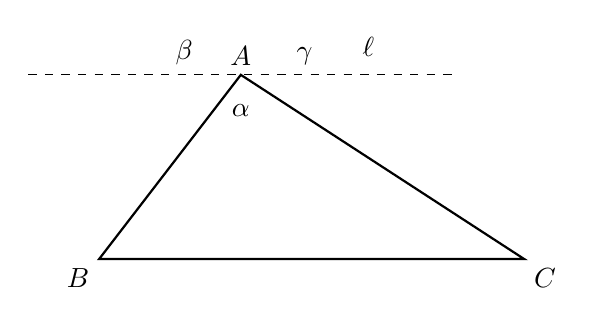
\begin{tikzpicture}[scale=0.9]
\draw[thick] (0,0) -- (6,0) -- (2,2.6) -- cycle;
\draw[dashed] (-1,2.6) -- (5,2.6);
\node[below left] at (0,0) {$B$};
\node[below right] at (6,0) {$C$};
\node[above] at (2,2.6) {$A$};
\node at (3.8,3.0) {$\ell$};
\node[above] at (1.2,2.6) {$\beta$};
\node[above] at (2.9,2.6) {$\gamma$};
\node at (2,2.1) {$\alpha$};
\end{tikzpicture}
\end{center}

\begin{proof}
设三角形为 $\triangle ABC$。过顶点 $A$ 作一条与边 $BC$ 平行的直线 $\ell$（即图中的虚线）。这条线不在原图里，是我们为了推理\textbf{加}进去的，所以叫辅助线。

边 $AB$ 同时穿过两条平行线 $\ell$ 与 $BC$，于是 $\ell$ 在 $A$ 点左侧与 $AB$ 形成的角 $\beta$ 等于角 $B$（内错角相等）；同理，$\ell$ 在 $A$ 点右侧与 $AC$ 形成的角 $\gamma$ 等于角 $C$。而在点 $A$ 处，$\beta$、角 $A$ 本身（图中的 $\alpha$）与 $\gamma$ 恰好拼成一个平角，也就是 $180^\circ$。所以
\[
\angle A+\angle B+\angle C=180^\circ.
\]
注意这个论证没有量任何一个角，它对每一个三角形都成立，无论边长多少。
\end{proof}

这个证明里最值得品味的动作是“作一条平行线”。图上本来没有它，是我们请来帮忙的客人。客人一到，角 $B$ 和角 $C$ 就被“搬”到了点 $A$ 旁边，三个角肩并肩站成一条直线，结论自己走了出来。辅助线是几何证明里最有创造性的部分：没有固定套路，靠的是对图形的理解和一点点运气。后面你还会看到它更多的表演。

\section{一条定理，两种理由}

现在轮到本章的主角登场。直角三角形是三角形里最特别的一类：有一个角恰好是 $90^\circ$。夹直角的两条边叫直角边，直角对着的最长边叫斜边。关于它有一条也许是全世界最著名的定理。

\begin{dingli}[勾股定理]
直角三角形两条直角边的平方和，等于斜边的平方。若直角边长为 $a$、$b$，斜边长为 $c$，则
\[
a^2+b^2=c^2.
\]
\end{dingli}

先看几个数。$3$、$4$、$5$：$9+16=25$，对。$5$、$12$、$13$：$25+144=169$，对。古埃及人拉绳子定直角时用的就是 $3$、$4$、$5$：把一根绳子打上等距的十二个结，围成三边为 $3$、$4$、$5$ 段的三角形，最大的角就是直角。但同样的问题又来了：验证一万组数，不等于证明了定理。下面给出两种完全不同的证明——同一个结论，两种不同的理由。这本身就是一个重要的数学事实：定理是被结论保证的，不是被某一种证法垄断的；多一种证法，就多一种理解。

\textbf{证法一：拼一拼面积。}

\begin{center}
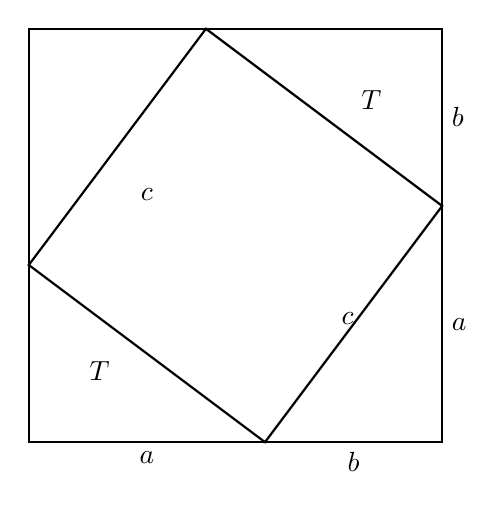
\begin{tikzpicture}[scale=0.75]
\draw[thick] (0,0) -- (7,0) -- (7,7) -- (0,7) -- cycle;
\draw[thick] (4,0) -- (7,4) -- (3,7) -- (0,3) -- cycle;
\node at (2,4.2) {$c$};
\node at (5.4,2.1) {$c$};
\node[below] at (2,0) {$a$};
\node[below] at (5.5,0) {$b$};
\node[right] at (7,2) {$a$};
\node[right] at (7,5.5) {$b$};
\node at (1.2,1.2) {$T$};
\node at (5.8,5.8) {$T$};
\end{tikzpicture}
\end{center}

\begin{proof}
取四个全等的直角三角形，直角边为 $a$、$b$，斜边为 $c$。把它们摆进一个边长为 $a+b$ 的大正方形里：每个三角形占据一个角，斜边朝内。四个斜边围出中间一个四边形。

先确认中间这块确实是正方形。它的四条边都是 $c$，只需再看一个角：在大正方形底边的拼接点处，一个三角形的锐角 $\alpha$、另一个三角形的锐角 $\beta$ 与中间四边形的角拼成平角 $180^\circ$，而 $\alpha+\beta=90^\circ$（它们是同一个直角三角形的两个锐角），所以中间那个角是 $90^\circ$。四边相等且有一个直角的菱形是正方形，面积为 $c^2$。

现在用两种方法算同一个大正方形的面积。直接算：$(a+b)^2$。拆开算：四个三角形加中间正方形，每个三角形面积为 $\frac{1}{2}ab$，所以
\[
(a+b)^2=4\times\frac{1}{2}ab+c^2=2ab+c^2.
\]
把左边展开：$a^2+2ab+b^2=2ab+c^2$，两边同时减去 $2ab$，得到 $a^2+b^2=c^2$。
\end{proof}

这个证明的灵魂是什么？是\textbf{面积在剪开和重新拼合中不变}。图形的形状变了，面积没有变——面积是剪拼操作下的“不变量”。抓住一个在变化中保持不变的量，常常是证明的钥匙，这个思想以后会反复出现。

\textbf{证法二：用相似。}

\begin{proof}
设直角三角形为 $\triangle ABC$，直角在 $C$，斜边为 $AB$。从 $C$ 向斜边 $AB$ 作垂线，垂足为 $D$——又是一条辅助线。这条垂线把原三角形劈成两个小三角形：$\triangle ACD$ 与 $\triangle CBD$。

比较 $\triangle ACD$ 和原来的 $\triangle ABC$：它们共用角 $A$，又各有一个直角（角 $ADC$ 与角 $ACB$），两角对应相等，所以相似。同理 $\triangle CBD$ 也与 $\triangle ABC$ 相似。写下对应边的比例。设 $AB=c$，$AC=b$，$BC=a$，$AD$ 记为 $x$，$BD$ 记为 $y$，注意 $x+y=c$。由 $\triangle ACD \sim \triangle ABC$（斜边对斜边，直角边 $AC$ 对直角边 $AD$）得
\[
\frac{AC}{AB}=\frac{AD}{AC},\quad\text{即 } b^2=cx.
\]
由 $\triangle CBD \sim \triangle ABC$ 同理得 $a^2=cy$。两式相加：
\[
a^2+b^2=cx+cy=c(x+y)=c^2.
\]
这里我们用到了“相似三角形对应边成比例”这条基本性质；它的严格证明需要更多准备，本章先把它当作约定的工具，就像下棋时先约定规则。
\end{proof}

请比较两种理由的“口味”。证法一把定理讲成面积的故事：$a^2$、$b^2$、$c^2$ 不再是抽象的平方，而是三块实实在在的、可以剪下来称重的正方形面积，勾股定理说的是“两块小正方形恰好能拼成斜边上的大正方形”。证法二把定理讲成形状的故事：直角三角形里藏着它自己的两个缩小版，自相似的结构迫使等式成立。两个证明都没有量任何长度，都对每一个直角三角形成立。

顺带一提，这个定理的证明可能有几百种：有靠梯形面积的，有靠圆的，还有纯代数配方和弦图的另一摆法（见思考题）。数学家们至今仍偶尔发表新的证明——不是因为旧证明不可靠，而是因为每种新理由都可能照亮定理的一个新侧面，并在别处派上用场。

\section{不变量、分类讨论和圆}

勾股定理的两个证明用了两件通用武器：不变量和辅助线。这一节把第三件武器也摆上桌面，然后让它们一起到圆那里去干活。

\textbf{分类讨论}的意思很朴素：当一个命题的条件可能对应几种不同情形时，把情形分干净，每种分别解决。前面“边边角”的反例里，一段圆弧和一条射线可能交出零个、一个或两个点，三种情形给出“不存在、唯一、两解”三种命运——不分类，就说不清。再比如判断三条线段能否围成三角形，只需用到下面这条从“两点之间线段最短”直接推来的事实。

\begin{tuilun}[三角形不等式]
三角形任意两边之和大于第三边。反过来，三条线段中若两条较短者之和大于最长者，它们就能围成一个三角形。
\end{tuilun}

注意这个推论自带分类思想：不用把三对边全查一遍，只查“最短两条加起来是否超过最长那条”这一种关键情形就够了。

\textbf{不变量}则是反过来问：图形在动，什么东西不动？剪拼时面积不动；放大缩小时角度不动、形状不动（这正是相似的全部内容）；而圆给了我们一个更漂亮的例子。

把圆定义为“到一个定点（圆心）距离等于定长（半径 $r$）的所有点”，然后看它的周长。拿绳子量几个圆：硬币、杯口、圆桌，你会发现周长除以直径总是大约 $3.14$。这又是测量带来的猜想。它为什么一定成立？因为任意两个圆都相似——把一个圆以任意点为中心放大，它还是一个圆。相似图形对应长度的比是固定的，于是“周长与直径之比”对所有圆都是同一个数。这个数就是 $\pi$。它是一个无理数，小数部分永远写不完，$3.14$ 或 $3.14159$ 都只是近似值。古人为了逼近它想出了绝妙的办法：在圆内作内接正多边形，边数越多，多边形周长越接近圆周。用正 $96$ 边形上下夹逼，可以把 $\pi$ 夹在 $3.1410$ 与 $3.1427$ 之间——这是阿基米德时代的成就，也是用有限逼近无限的第一次胜利，第十一章讲极限时我们还会回到这个画面。

\begin{shuyu}{不变量}
直观解释：大家都在变，它偏不变，所以它能当“标尺”和“证人”。
正式定义：在某种操作或变换下保持不变的量或性质。
例子：剪纸重拼时面积不变，所以可以用“两种摆法算同一面积”来证明勾股定理。
\end{shuyu}

面积本身也值得一个定义。严格定义面积并不容易（第十二章的积分才会真正对付它），但在初中阶段我们可以约定：边长为 $1$ 的正方形面积为 $1$，面积在剪拼下可加、不变。由此推出矩形面积是长乘宽，平行四边形面积是底乘高（剪下一个直角三角形挪到另一边就拼成矩形），三角形面积是底乘高的一半（两个全等三角形拼成平行四边形），圆面积是 $\pi r^2$（把圆切成很多小扇形交错拼成近似的矩形，长为半周长 $\pi r$、宽为 $r$——这又是逼近思想的预演）。每一条公式背后都站着一次剪拼，而不是一次测量。

\begin{toolbox}
本章添置的新工具：
\begin{itemize}
\item \textbf{公理与定义}：推理的起点不是“是什么”，而是“遵守什么规则”；先把“一样”拆成全等与相似。
\item \textbf{全等、相似判定}：不必叠在一起比较，核对恰当的两三个条件即可锁定形状。
\item \textbf{辅助线}：图上没有的线可以请来帮忙，平行线负责搬角，垂线负责制造直角与相似。
\item \textbf{分类讨论}：条件对应多种情形时，分干净、逐个击破；边边角的陷阱就是漏分类的下场。
\item \textbf{不变量}：剪拼中的面积、缩放中的角度、所有圆共享的 $\pi$——抓住不变的量，变化就有了把柄。
\item \textbf{测量与证明的分工}：测量负责发现猜想、提供例证，证明负责为“所有情形”签字画押。
\end{itemize}
\end{toolbox}

\section{换一种眼光：三角测量与星空}

几何学最壮观的应用，恰恰建立在它最抽象的结论上。古希腊人想知道月亮有多远、太阳有多远，他们手里没有火箭，只有相似三角形和角度。

思路今天还在用，叫三角测量：要测一个到不了的点 $C$，先在选好的两个点 $A$、$B$ 量出基线长度 $AB$，再分别量出视线 $AC$、$BC$ 与基线的夹角。三角形 $\triangle ABC$ 被“两角夹一边”完全锁定，虽然 $C$ 远在天边，它的形状却是确定的。画一个按比例缩小的副本，或者用相似与比例计算，$AC$、$BC$ 就出来了。测量员测河对岸的塔、测绘队画全国地图、天文学家用地面上两个观测站对准月球，用的都是同一招。到了更晚的时代，人们还试着用地球本身当基线去量行星的距离。

注意这个应用的前提：我们相信“两角夹一边唯一决定三角形”“相似三角形对应边成比例”这些命题对地面上、月球那么大的三角形同样成立。如果这些命题只是“量过很多小三角形都对”的经验，把结论外推到天文尺度就是一场豪赌；正因为它们是定理，工程师和天文学家才敢把身家性命押上去。这就是证明的实用价值——它不是书斋里的洁癖，而是让知识可以放大到任何尺度的许可证。

\begin{lianjie}
回头看：第 1 章的字母和比例，在本章变成了相似比与面积公式；第 2 章的方程，让我们能从 $a^2+b^2=c^2$ 里解出未知边。往前看：本章始终在一个没有名字的平面上画图，点只有位置、没有“地址”。下一章我们将给每个点发一张写着两个数的身份证——坐标。到那时，直线、圆都会变成方程，几何题可以用代数算，代数式也可以画出形状。你即将看到本章的定理（尤其是勾股定理）变成坐标世界里最忙的公式：距离公式。
\end{lianjie}

\section{动手做一做}

\begin{shiyan}
\textbf{实验一：绳结直角。} 找一根软绳，用记号笔打上 $12$ 个等距的结。把绳子围成三边分别为 $3$、$4$、$5$ 段间隔的三角形，拉紧，用三角板的直角去比最大的那个角。再试试 $5$、$12$、$13$ 段（需要 $30$ 个间隔）。想一想：你为什么相信拉紧后得到的是直角——这是测量结论还是定理结论？

\textbf{实验二：剪纸证勾股。} 在方格纸上画一个直角边为 $3$ 格、$4$ 格的直角三角形，再复印三份（或照画三个全等的）。按本章证法一的摆法，把四个三角形摆进一个 $7\times7$ 的方格里，数一数中间空出的正方形占几格。$49-4\times6=25$，正好是 $5\times5$。再换一组直角边（比如 $2$ 格、$5$ 格）重做一遍，验证中间面积是否为 $2^2+5^2=29$ 格。

\textbf{实验三：逼近 $\pi$。} 用圆规画一个半径 $5$ 厘米的圆，用直尺在圆内依次作内接正六边形、正十二边形（把每条弧用中点劈开），量出多边形周长，除以直径 $10$ 厘米，记录结果如何向 $3.14$ 靠近。注意：无论你量得多仔细，这一步永远只是测量；$\pi$ 的精确性质要靠推理。
\end{shiyan}

\section*{思考题}

\textbf{观察题}
\begin{sikao}
\item 画三个形状差别很大的三角形（一个瘦高、一个扁宽、一个接近等边），量各自的三个内角并求和，把每次的偏差记下来。偏差有正有负还是总朝一边？提示：想想量角器的最小刻度和你的读数习惯，误差从哪里来。
\item 同一根竖直旗杆，在一天的不同时刻量它的影长，算一算“杆高除以影长”是否变化。提示：什么时候这个比值相同？什么在变化、什么是不变量？
\end{sikao}

\textbf{证明题}
\begin{sikao}
\item 弦图还有另一种摆法：把四个全等的直角三角形（直角边 $a$、$b$，$a<b$）摆进一个边长为 $c$ 的大正方形里，使斜边贴着大正方形的四条边，中间空出一个小正方形。提示：中间小正方形的边长是 $b-a$，用两种方法算大正方形面积。
\item 证明：等腰三角形的两个底角相等。提示：作顶角的平分线（或底边上的高），把三角形分成两块，用全等判定说明两块全等。
\end{sikao}

\textbf{挑战题}
\begin{sikao}
\item 证明：圆内接三角形中，若一条边是直径，则这条边所对的角是直角。提示：连接圆心与这个角的顶点，圆被分成两个等腰三角形，给四个底角起两个名字，再用内角和。
\item 两千多年前，有人利用“夏至正午，某城太阳光直射井底（影长为零），同一时刻北方另一城的杆影偏角约为圆周的五十分之一，而两城距离已知”算出了地球的周长。提示：把太阳光当作平行线，两座城和地心构成什么图形？杆影的偏角等于哪个圆心角？你需要哪些假设，其中哪一条只是近似成立？
\end{sikao}

\begin{pandeng}
本章的图景在两千多年前被系统地整理进一部叫《几何原本》的书里：从五条公理出发，推出几百条定理，这种“公理化”的写法至今仍是数学的硬通货。继续向前，你会遇到这些关键词：欧几里得第五公设（平行公理）与非欧几何——换掉它，三角形内角和就不再是 $180^\circ$；射影几何——研究透视与影子本身的学问；三角学——把相似三角形浓缩成正弦、余弦两张函数表；解析几何——下一章的起点，用方程驯服曲线；以及现代的几何证明自动化与计算机辅助证明，机器也能当几何学家。
\end{pandeng}

\section*{通往下一章的门}

这一章我们学会了在一张白纸上证明事情：作辅助线、找全等、用相似、抓不变量。但你可能注意到了一个隐隐的不便——纸上的点没有名字。我们说“斜边上的垂足”，说“圆心右侧三厘米处”，全靠手势和形容词。如果一个几何问题里有一百个点、二十条曲线呢？如果你想让一台没有眼睛的计算机帮你画图、验证猜想呢？它听不懂“左边那个点”，它只认数。

于是有一个朴素到近乎幼稚的问题浮上来：能不能给平面上的每一个点起一个由数字组成的名字？一旦做到，“两点之间的距离”会变成一道算术题，“直线”和“圆”会变成方程，本章所有的定理将拥有一种新的语言。下一章，我们就去建这座桥——从勾股定理出发，给平面装上坐标。
